\documentclass[xcolor=dvipsnames]{beamer}
%\documentclass[handout,xcolor=dvipsnames,pdftex,hyperref={colorlinks=false}]{beamer}
\usetheme[height=7mm]{Rochester}
\setbeamertemplate{items}[ball]
\setbeamertemplate{blocks}[rounded][shadow=true]
\usepackage{xcolor}
\usepackage{colortbl}
\usepackage{multirow}
\usepackage{amsmath,amsthm,amssymb}
\usepackage{amsfonts}
\usepackage{epsfig}
\usepackage{times}
\usepackage[T1]{fontenc}
\usepackage{inconsolata}
\usepackage{fancyvrb}
\usepackage{bbm}
\usepackage{subcaption}
\usepackage[normalem]{ulem}

\newcommand{\Plus}{\mathord{\tikz\draw[line width=0.3ex, x=1ex, y=1ex] (0.5,0) -- (0.5,1)(0,0.5) -- (1,0.5);}}


\newcommand{\lra}{\leftrightarrow}
\newcommand{\ra}{\rightarrow}
\newcommand{\la}{\leftarrow}
\newcommand{\mc}{\mathclap}

\usepackage{tikz}
\usetikzlibrary{positioning}
\usetikzlibrary{shapes,decorations,arrows,calc,arrows.meta} 
\tikzset{
	-latex,auto,node distance = 1.5cm and 1.5cm,
	semithick ,
	state/.style ={ellipse, draw, minimum width = 0.5 cm},
    old inner xsep/.estore in=\oldinnerxsep,
    old inner ysep/.estore in=\oldinnerysep,
	el/.style = {inner sep=2pt, align=left, sloped},
	point/.style = {circle, draw=black, inner sep=0.04cm,
	 fill=black,
                node contents={}},
}

% == theme & colors
\usetheme{Warsaw}  % Jens' previous
%\usepackage{helvet}
\definecolor{someblue}{rgb}{0,.1,0.8}

\title{Stat 256: Causality}
\date{Spring 2026}
\subtitle[ ]{Causal Graphs and Causal Structural Models}
\author{Chad Hazlett}
\institute[UCLA]{UCLA\\[1ex]
  \texttt{chazlett@ucla.edu}}

\definecolor{dgreen}{rgb}{0,.6,0.8}
\newtheorem{assumption}{Assumption}
\newtheorem{arule}{Rule}
\newtheorem{iass}{Identification Assumption}
\newtheorem{ires}{Identification Result}
\newtheorem{estm}{Estimand}
\newtheorem{esti}{Estimator}
\newtheorem{question}{Question}
\newtheorem{answer}{Answer}
\newtheorem{proposition}{Proposition}
\newtheorem{corrolary}{Corollary}

\newcommand{\bs}{\boldsymbol}
\newcommand{\mb}{\mathbf}
\newcommand{\real}{\mathbb{R}}
\renewcommand{\u}{\ensuremath{\mb{u}}}
\renewcommand{\v}{\ensuremath{\mb{v}}}
\newcommand{\U}{\ensuremath{\mb{U}}}
\newcommand{\Z}{\ensuremath{\mb{Z}}}
\newcommand{\PP}{\ensuremath{\mb{P}}}
\newcommand{\M}{\ensuremath{\mb{M}}}
\newcommand{\X}{\ensuremath{\mb{X}}}
\newcommand{\x}{\ensuremath{\mb{x}}}
\newcommand{\Y}{\ensuremath{\mb{Y}}}
\newcommand{\D}{\ensuremath{\mb{D}}}
\newcommand{\y}{\ensuremath{\mb{y}}}
\renewcommand{\b}{\ensuremath{\bs{\beta}}}
\newcommand{\e}{\ensuremath{\bs{\epsilon}}}
\newcommand{\bhat}{\ensuremath{\hat{\bs{\beta}}}}
\newcommand{\XX}{\ensuremath{\X'\X}}
\newcommand{\XXinv}{\ensuremath{\left(\XX\right)^{-1}}}
\newcommand{\hatsig}{\ensuremath{\hat{\sigma}^2}}
\newcommand{\sig}{\ensuremath{\sigma^2}}
\newcommand{\hatmat}{\ensuremath{\X \XXinv \X'}}
\newcommand{\ehat}{\ensuremath{\hat{\e}}}
\newcommand{\tr}{\text{tr}}
\newcommand{\Sig}{\ensuremath{\bs{\Sigma}}}
\newcommand{\SigInv}{\ensuremath{\bs{\Sigma^{-1}}}}
\newcommand{\W}{\ensuremath{\mb{W}}}
\newcommand\E{\mathbb{E}}

\newcommand{\indep}{{\bot\negthickspace\negthickspace\bot}}
%\newcommand{\indep}{\mbox{$\bot\!\!\!\bot$}}


\useoutertheme{infolines}
\begin{document}


\subject{Talks}
\AtBeginSection[]
{
  \begin{frame}<beamer>
    \frametitle{Outline}
    \tableofcontents[currentsection]
  \end{frame}
}

\AtBeginSubsection[]
{
  \begin{frame}<beamer>
    \frametitle{Outline}
    \tableofcontents[currentsection,currentsubsection]
  \end{frame}
}

\begin{frame}
  \titlepage
\end{frame}

\begin{frame}{Resources for this material}

\onslide<1-> Today we will just get our feet wet, but for the DAG material in general:\\
\bigskip
\onslide<1-> Required reading:\\
\begin{itemize}
\item  \textit{What if} (Hernan and Robins), Chapters 6, 7.
\item  \textit{Primer} (Pearl, Glymour, Jewell), Chapters 1.4, 1.5, 2, 3.
\end{itemize}

\onslide<2-> Other suggestions:\\
\begin{itemize}
\item  Pearl, J. (2009).  \textit{Causality} \\
\item<3-> Some online materials:\\
\begin{itemize}
\item \textit{Causal Diagrams: Draw Your Assumptions Before Your Conclusions} course by Miguel Hernan on EdX
\item \textit{A Crash Course in Causality: Inferring Causal Effects from Observational Data} course by Jason Roy on Coursera.
\item Richard McElreath lecture on ``Science before statistics: causal inference''. \url{https://www.youtube.com/watch?v=KNPYUVmY3NM&t=8565s}
\end{itemize}
\end{itemize}
\end{frame}

\begin{frame}{Goals for this lecture}
\begin{itemize}
\item<1-> Motivation: Why do we need causal structure to make sense of data?
\bigskip
\item<2-> Introduction to structural causal models (SCMs) and their graphs
\bigskip
\item<3-> Graph basics: Conditional independence and $d$-separation
\end{itemize}
\end{frame}

\begin{frame}{Why we need causal structure}
\normalsize
\onslide<1-> Suppose people self-select into taking a new drug. You find: \\
\pause
\begin{table}[]
\begin{tabular}{lll}
                              & \multicolumn{2}{c}{Outcome:  Recovery}                                                                  \\
                              & Drug                                               & No Drug                                            \\ \cline{2-3}
\multicolumn{1}{l|}{Mild}     & \multicolumn{1}{l|}{81 of 87 (93\%)}   & \multicolumn{1}{l|}{234 of 270  (87\%)} \\ \cline{2-3}
\multicolumn{1}{l|}{Severe}   & \multicolumn{1}{l|}{192 of 263 (73\%)} & \multicolumn{1}{l|}{55 of 80  (69\%)}   \\ \cline{2-3}
\multicolumn{1}{l|}{Combined} & \multicolumn{1}{l|}{273 of 350 (78\%)}  & \multicolumn{1}{l|}{289 of 350 (83\%)} \\ \cline{2-3}
\end{tabular}
\end{table}

\small
\begin{itemize}
\item<3-> Among mild cases, those on the drug did better (93\% vs. 87\%)
\item<4-> Among severe cases, those on the drug did better (73\% vs. 69\%)
\item<5-> But in the combined data, people did \textit{worse} on the drug (78\% vs. 83\%)
\end{itemize}
\onslide<6-> Which comparison answers the causal question?
\end{frame}

\begin{frame}{What's going on? Confounding}
\begin{table}[]
\begin{tabular}{lll}
                              & \multicolumn{2}{c}{Outcome:  Recovery}                                                                  \\
                              & Drug                                               & No Drug                                            \\ \cline{2-3}
\multicolumn{1}{l|}{Mild}     & \multicolumn{1}{l|}{81 of 87 (93\%)}   & \multicolumn{1}{l|}{234 of 270  (87\%)} \\ \cline{2-3}
\multicolumn{1}{l|}{Severe}   & \multicolumn{1}{l|}{192 of 263 (73\%)} & \multicolumn{1}{l|}{55 of 80  (69\%)}   \\ \cline{2-3}
\multicolumn{1}{l|}{Combined} & \multicolumn{1}{l|}{273 of 350 (78\%)}  & \multicolumn{1}{l|}{289 of 350 (83\%)} \\ \cline{2-3}
\end{tabular}
\end{table}
\medskip
\small
\begin{itemize}
\item<2-> Severe cases have lower recovery rates \textit{and} are more likely to take drug.
\item<4-> So the drug group is disproportionately severe cases, dragging down its average --- classic confounding.
\end{itemize}
\onslide<5-> Knowing to condition on severity here required a causal judgment: that severity is a common cause of drug-taking and recovery. \\
\medskip
\onslide<6-> Thus knowing what to do -- and the answer you get -- depends on the analyst's beliefs about causal structure.\\
\end{frame}

\begin{frame}{Encoding causal assumptions}
\onslide<1-> In this example, our assumption is:
\footnotesize
\begin{enumerate}
\item Severity influences both recovery and drug-taking, and
\item no other factor creates a spurious association between drug-taking and recovery.
\end{enumerate}
\normalsize
\onslide<2-> We encode this with a DAG:\\
\begin{center}
    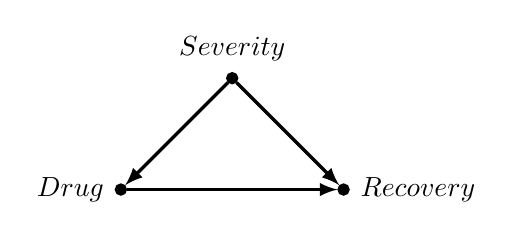
\begin{tikzpicture}[node distance = 2cm, very thick]
               \node (Severity)  [label = above:$Severity$,point];
                \node (Drug) [label = left:$Drug$ ,below left of = Severity , point];
                \node (Recovery) [label = right:$Recovery$ ,below right of = Severity, point];
                \path (Severity) edge  (Drug);
               \path (Severity) edge  (Recovery);
                \path (Drug) edge  (Recovery);
        \end{tikzpicture}
 \end{center}
\small
\onslide<3-> Preview: this graph  shows us that conditioning on Severity removes the confounding,  isolates the effect of Drug on Recovery. \\
%\medskip
%\onslide<4-> \small Later, we will see how potential outcomes encode similar assumptions differently --- and how the two frameworks connect.
\end{frame}

%\begin{frame}{The bigger picture}
%\small
%\onslide<1-> We need a language that allows us to (i) express our causal assumptions, (ii) make causal queries, (iii) determine if those queries can be answered; (iv) tell us how to get those answers.  \\
%\medskip
%\begin{enumerate}
%\item<2-> We will rely on \textcolor{Blue}{structural causal models} and (mainly) their graphical  representations as \textcolor{Blue}{Directed Acyclic Graphs}. 
%\medskip
%\item<3-> \textcolor{Blue}{Potential outcomes} and counterfactuals can be said to be produced by these models, describing outcomes under particular interventions. Another tradition begins with assumptions on these. 
%\medskip
%%\item make some things easier and somethings harder; clarify some assumptions and obscure others
%\item<4-> These traditions are all of a piece, and have different strengths and weakneses... we will practice going back and forth between them.
%\end{enumerate}
%\end{frame}

\begin{frame}{Structural Causal Models}
\onslide<1-> Let's now formalize what we mean by ``causal structure.'' \\
\medskip
\onslide<2-> Structural Causal Models (SCMs) specify a set of causal relationships.   They consist of:\\
\footnotesize
\begin{itemize}
\item a group of observed variables 
\item a group of unobserved exogenous variables, $\{U\}$
\item functions that relate them, $f_{(\cdot)}$
\item  an assumed distribution over the exogenous variables, $p(U)$.
\end{itemize}
\onslide<2->  E.g.,
            \begin{align*}
                X &= f_{x}(U_x)\\
                A &= f_{a}(X, U_a)\\
                Y &= f_{y}(X, A, U_y)\\
                U_{y}&\indep U_{x},~ U_{y}\indep U_{a}
            \end{align*}
          
where ``exogenous'' ancestors,  $U = \{U_{x}, U_{a}, U_{y}\}$ with $U\sim p(u)$.  
\end{frame}

\begin{frame}{Life in an SCM}

\onslide<1-> Note that:
\footnotesize
\begin{itemize}
\item $\{f_{x}, f_{a}, f_{y}\}$ make no parametric commitments.
\item Each expression has a causal ("structural") meaning, not just algebraic.
\item ``$X$ causes $Y$'' means $Y$'s function depends on $X$
\end{itemize}
\medskip
\normalsize
\onslide<2-> SCMs impose a deterministic, ``clockwork'' notion of causation:\\
\footnotesize
\begin{itemize}
\item<3-> Population: The distribution $p(U)$ implies a distribution $p(\text{observables})$.
\item<4-> Individuals: If you knew all the values of $U$ for a given unit and the details of every $f$, you would know the exact values of every variable.
\item<5-> Modularity/invariance: each function $f_j$ does not depend on how its inputs were produced. If you \textit{intervene} and set $A=a$, the downstream functions still apply as usual. We will use this when we discuss interventions.
\end{itemize}
\end{frame}

\begin{frame}{SCM to Graph}
\small
%\onslide<1-> In this context, ``$X$ causes $Y$'' means $Y$'s function depends on $X$. Pearl puts it nicely (\textit{Primer}): ``$X$ is a cause of $Y$ if $Y$ listens to $X$ and decides its value in response to what it hears.''  \\
%\bigskip
%\small
For a model $M$ such as:
            \begin{align*}
                X &= f_{x}(U_x)\\
                A &= f_{a}(X, U_a)\\
                Y &= f_{y}(X, A, U_y)\\
                U_{y}&\indep U_{x},~ U_{y}\indep U_{a}
            \end{align*}
          
It is convenient to draw a graph, $G$:
\onslide<2->\\
\begin{center}
            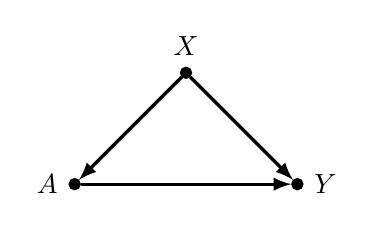
\begin{tikzpicture}[node distance = 2cm, very thick]
               \node (x)  [label = above:$X$,point];
                \node (a) [label = left:$A$ ,below left of = x , point];
                \node (y) [label = right:$Y$ ,below right of = x, point];
                % \node (u) [label = below:$(U)$ ,below right of = x, point, color = red];
                %\path[latex-latex, dashed] (z) edge[bend right = 50]  (x);
                \path (x) edge  (a);
               \path (x) edge  (y);
                \path (a) edge  (y);
                % \path (u) edge[color = red] node[below, el, color = black] {$\lambda_{ux}$} (x);
            %    \path (u) edge[color = red] node[below, el, color = black] {$\lambda_{uy}$} (y);
            % \caption{Graph $G(M)$}
        \end{tikzpicture}
 \end{center}
        \footnotesize
        \begin{itemize}
        \item<3->  Arrows go into a node only if the corresponding argument enters the corresponding function in the SCM.
        \item<4-> You could show $U_j$ pointing to each $j$, but usually omit these. 
        \end{itemize}
\end{frame}


\begin{frame}{Missing edges, bidirected arcs}
\small        
        \onslide<1-> A missing edge means the value of $A$ is not an argument into $Y$. \textit{It's the missing edges that matter for the arguments we will need to make.}\\
        \bigskip
                \onslide<2-> Some authors show unobserved common causes as a bidirected arc. \\
        \bigskip
        \begin{center}
  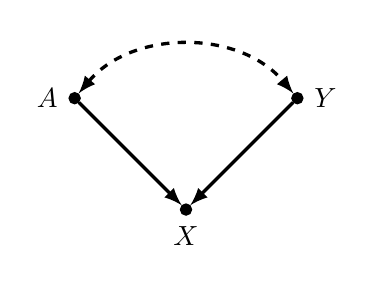
\begin{tikzpicture}[node distance = 2cm, very thick]
               \node (x)  [label = below:$X$,point];
                \node (a) [label = left:$A$, above left of = x , point];
                \node (y) [label = right:$Y$ ,above right of = x, point];
                % \node (u) [label = below:$(U)$ ,below right of = x, point, color = red];
                \path[latex-latex, dashed] (a) edge[bend left = 50]  (y);
                \path (a) edge  (x);
               \path (y) edge  (x);
        \end{tikzpicture}
\end{center}
\end{frame}

\begin{frame}{Terminology}
\begin{enumerate}
\item<1-> nodes, vertices: the variables that are written
\item<2-> edges, arrows: the lines,  may be ``directed'' or ``bidirected'' (arcs)
\item<3-> parents: for a given node, the causes feeding into it
\item<4-> root nodes: a node with no (endogenous) parents on the graph
\item<5-> descendants, children: effects of a given cause
\item<6-> paths: any series of connected nodes, regardless of direction
\item<6-> \textbf{D}irected \textbf{A}cyclic \textbf{G}raph: a graph where all edges are directed and you can never follow directed paths from a node back to itself.
\end{enumerate}
\end{frame}

\begin{frame}{Factorization}
\small
\textcolor{blue}{Markov condition}: Each node listens only to its parents. For some node $X$, its parents ($PA$) and non-parent, non-descendants $Q$, 
$$p(X|PA, Q) = p(X|PA)$$\\
\medskip
\onslide<2-> We'll often use this to see what should be conditionally independent,  
\[ X \indep Q \mid PA  \]\\

\onslide<3-> Further, this allows ``Markov factorization'' of the joint distribution:
\begin{arule}
\footnotesize
Product Decomposition (Pearl \& Verma 1991):  for any model $M$ whose graph $G$ is acyclic and without dependent unobserved causes (i.e. no bidirected arcs; Markovian), the joint distribution of variables in the model is given by
\[ P(X_1, X_2, ... , X_n) =  \prod_i P(X_i | PA_i)  \]
where $PA_i$ denotes the parents of $X_i$
\end{arule}
\end{frame}

\begin{frame}{Example of Product Decomposition}
\begin{center}
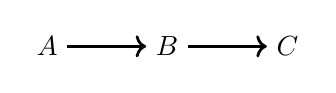
\begin{tikzpicture}
\node[text centered] (A) {$A$};
\node[right = 1 of A, text centered] (B) {$B$};
\node[right=1 of B, text centered] (C) {$C$};
% edges %
\draw[->, line width= 1] (A) --  (B);
\draw [->, line width= 1] (B) -- (C);
\end{tikzpicture}
\end{center}

\small
What is $P(A,B,C)$?  \\
\medskip
\onslide<2-> Without the graph, you could always write
\[ P(A, B, C) = P(A) P(B|A) \textcolor{blue}{P(C|B, A)}  \] 
\medskip 
\onslide<3-> With the graph we can write:\\
\[ P(A, B, C) = P(A) P(B|A) \textcolor{blue}{P(C|B)}  \] 
\end{frame}

\begin{frame}{Paths, dependencies, and information}  
\onslide<1-> A first use of graphs is to get a handle on what observables will be conditionally or marginally associated with what others. \\

\medskip

\onslide<2-> Three key structures: forks, chains, colliders \\

\medskip

\onslide<2-> \textcolor{blue}{Chain}:
\begin{center}
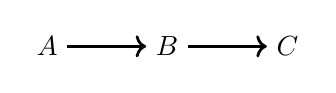
\begin{tikzpicture}
\node[text centered] (A) {$A$};
\node[right = 1 of A, text centered] (B) {$B$};
\node[right=1 of B, text centered] (C) {$C$};
% edges %
\draw[->, line width= 1] (A) --  (B);
\draw [->, line width= 1] (B) -- (C);

\end{tikzpicture}
\end{center}

\onslide<3-> Implications:\\
\medskip
 \onslide<4-> $A \indep C$ ? \onslide<5-> \textcolor{Red}{No} --- $A$ influences $C$ through $B$. \\
 \medskip
\onslide<6-> $A \indep C | B$? \onslide<7-> \textcolor{Green}{Yes} --- conditioning on $B$ blocks the chain.\\
\medskip
\onslide<8-> $ B \indep C | A $? \onslide<9-> \textcolor{Red}{No} --- $B$ still directly causes $C$.
\end{frame}

\begin{frame}{Paths, dependencies, and information}

\onslide<1-> \textcolor{blue}{Fork} (aka common cause): 
\begin{center}
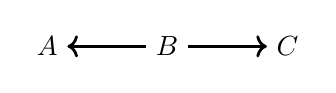
\begin{tikzpicture}
\node[text centered] (A) {$A$};
\node[right = 1 of A, text centered] (B) {$B$};
\node[right=1 of B, text centered] (C) {$C$};
% edges %
\draw[->, line width= 1] (B) --  (A);
\draw [->, line width= 1] (B) -- (C);
\end{tikzpicture}
\end{center}

\onslide<2-> Implications:\\
\medskip
 \onslide<3-> $A \indep C$ ? \onslide<4-> \textcolor{Red}{No} --- the common cause $B$ induces association.\\
 \medskip
\onslide<5-> $A \indep C | B$? \onslide<6-> \textcolor{Green}{Yes} --- conditioning on the common cause blocks it.\\
\medskip
\onslide<7-> $ B \indep C | A $? \onslide<8-> \textcolor{Red}{No} --- $B$ still directly causes $C$.
\end{frame}

\begin{frame}{Paths, dependencies, and information}

\onslide<1-> \textcolor{blue}{Collider}: 
\begin{center}
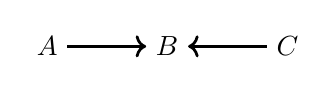
\begin{tikzpicture}
\node[text centered] (A) {$A$};
\node[right = 1 of A, text centered] (B) {$B$};
\node[right=1 of B, text centered] (C) {$C$};
% edges %
\draw[->, line width= 1] (A) --  (B);
\draw [->, line width= 1] (C) -- (B);
\end{tikzpicture}
\end{center}

\medskip
 \onslide<2-> $A \indep C$ ? \onslide<3-> \textcolor{Green}{Yes} --- no common cause, no causal path.\\
 \medskip
\onslide<4-> $A \indep C | B$? \onslide<5-> \textcolor{Red}{No!} --- conditioning on the collider \textit{opens} a path.\\
\medskip
\onslide<6-> $ B \indep C | A $? \onslide<7-> \textcolor{Red}{No} --- $C$ directly causes $B$.
\begin{center}
\onslide<5-> \textcolor{Red}{Beware colliders!}
\end{center}
\end{frame}

\begin{frame}{Colliding is real}
 \footnotesize
\onslide<1-> Pearl's favorite ($A \ra B \la C$): \\
\begin{itemize}
\item[] A: It rains
\item[] B: The lawn is wet (collider)
\item[] C: Sprinkler recently on
\end{itemize}
\bigskip
\onslide<2-> Hollywood success ($A \ra B \la C$):\\
\begin{itemize}
\item[] A: Good looks
\item[] B: Fame (collider)
\item[] C: Acting skills
\end{itemize}
\bigskip
\onslide<3-> Academic tenure ($A \ra B \la C$):\\
\begin{itemize}
\item[] A: Productivity
\item[] B: Tenure (collider)
\item[] C: Originality\footnote{Thanks to Jason Roy for these examples}
\end{itemize}
\end{frame}

\begin{frame}
\begin{figure}[h!]
\begin{center}
\includegraphics[scale=0.45]{Free Throw Percentage vs Height.png}
\end{center}
\end{figure}

\onslide<2-> Why do you think that is? Answer with a DAG. \\
\medskip
\footnotesize
*Source: Adam Rohde, via \url{https://www.basketball-reference.com/} and \url{https://www.kaggle.com/datasets/drgilermo/nba-players-stats}.
\end{frame}


\begin{frame}{$d$-Separation}
\small 
You now also understand  $d$ (directional)-Separation, which just follows from these to formalize when we can claim conditional independence

\onslide<2->
\begin{arule}
\textbf{$d$-separation}. \\ $A$ and $C$ are $d$-separated by a set of nodes $Z$ if and only if \textit{every path} between $A$ and $C$ is blocked, where a path is blocked if:\\
\begin{itemize}
\item it contains a chain ($\rightarrow B \rightarrow$) or fork ($\leftarrow B \rightarrow$) and $B \in Z$ (conditioning blocks it), or
\item it contains a collider ($\rightarrow B \leftarrow$) and neither $B$ nor any descendant of $B$ is in $Z$ (not conditioning keeps it closed).
\end{itemize}
\end{arule}

\onslide<3->  If $A$ and $C$ are $d$-separated by $Z$, then $A \indep C \mid Z$ in any distribution generated by that graph. \\
\end{frame}

%\begin{frame}{Preview: independence $\neq$ ignorability}
%\onslide<1-> Conditional \textcolor{blue}{independence} is about observables:
%$$D \indep Y \mid X$$
%This is what $d$-separation lets us read off a graph. \\
%\medskip
%\onslide<2-> Later, when we introduce potential outcomes, you will encounter conditional \textcolor{Green}{ignorability}:
%$$D \indep Y_d \mid X$$
%which involves \textit{counterfactual} quantities $Y_d$, not just observables. \\
%\medskip
%\onslide<3-> These are different concepts, but deeply connected: the conditional independence structure encoded in a DAG will be what lets us argue for conditional ignorability when we need it.
%\end{frame}

\begin{frame}{Practice}
\begin{center}
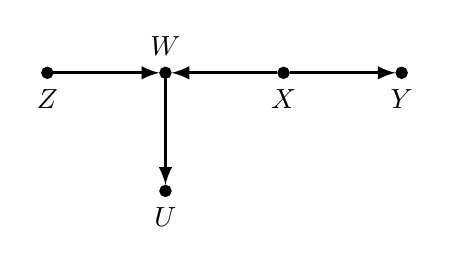
\begin{tikzpicture}[very thick]
	\node (z)  [label = below:$Z$, point];
	\node (w) [label = above:$W$ ,right of = z , point];
    \node (x) [label = below:$X$ , right of = w, point];
    \node (y) [label = below:$Y$ ,right of = x , point];
   \node (u) [label = below:$U$ ,below of = w, point];
             \path (z) edge  (w);
               \path (x) edge  (w);
                \path (w) edge  (u);               
               \path (x) edge  (y); 
\end{tikzpicture}
\end{center}

\onslide<2->  Looking at $Z$ and $Y$:
\begin{itemize}
\item Are they $d$-separated conditional on $\{\}$?
\item Are they $d$-separated conditional on $W$?
\item Are they $d$-separated conditional on $\{W,X\}$?
\item Are they $d$-separated conditional on $U$?
\end{itemize}
\end{frame}

\begin{frame}{More practice}
\begin{center}
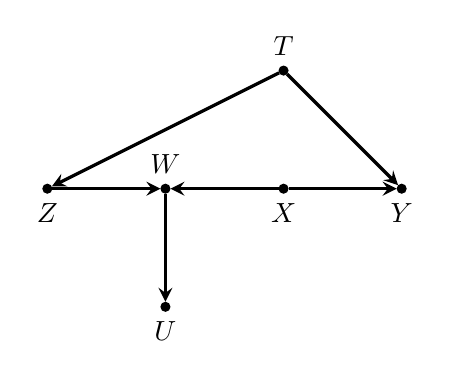
\begin{tikzpicture}
	\node (z)  [label = below:$Z$, point];
	\node (w) [label = above:$W$ ,right of = z, point];
    \node (x) [label = below:$X$, right of = w, point];
    \node (y) [label = below:$Y$ , right of = x , point];
   \node (u) [label = below:$U$ , below of = w , point];
   \node (t) [label= above:$T$, above of = x, point];
   \draw[->, >=stealth, very thick] (z) --  (w);
   \draw[->, >=stealth, very thick] (x) -- (w);
      \draw[->, >=stealth, very thick] (w) -- (u);
   \draw[->, >=stealth, very thick] (x) -- (y);
   \draw[->, >=stealth, very thick] (t) -- ( z);
   \draw[->, >=stealth, very thick] (t) -- (y);
\end{tikzpicture}
\end{center}

\onslide<2-> What sets $d$-separate $Z$ from $Y$?
\end{frame}


\begin{frame}{Review so far}
All of this is really to say that for two nodes of interest,\\
\begin{itemize}
\item<2-> they come to be associated due to (i) one causing another (directly or through a chain), (ii) a common cause; (iii) conditioning on a common consequence (collider) 
\smallskip
\item<3-> you can render them independent according to the rules of $d$-separation:
\begin{itemize}
\item if they are independent already
\item if you block the common cause or intermediate causal path by conditioning
\item if you don't condition on collider (or descendant thereof)
\end{itemize}
\item<4-> $d$-separation guarantees conditional independence; non-d-separation risks lack of independence.
\item<5-> This will lead to more interesting things soon, I promise!
\end{itemize}
\end{frame}

\end{document}
